% ============================================================
%  Semaine 2 — Fiche TP — Squelette HTML du MiniForum
%  cfpt·i | Anne Terrier
%  Charte graphique : charte cfpt·i originale, police sans-serif
% ============================================================
\documentclass[a4paper,11pt]{article}

\usepackage[T1]{fontenc}
\usepackage[utf8]{inputenc}
\usepackage[scaled=0.92]{helvet}
\renewcommand{\familydefault}{\sfdefault}
\usepackage[top=2.5cm, bottom=2.5cm, left=2.5cm, right=2.5cm, headheight=40pt]{geometry}
\usepackage{microtype}

\usepackage[dvipsnames,svgnames,table]{xcolor}
\usepackage{graphicx}
\usepackage{tikz}
\usetikzlibrary{positioning, arrows.meta, fit, backgrounds}

% --- Style commun des maquettes (fenêtre navigateur) ---
\newcommand{\browserbar}[1]{%
  \fill[cfptGrey] ([yshift=-0.02cm]#1.north west) rectangle ([yshift=-0.62cm]#1.north east);
  \draw[cfptDarkGrey!45] ([yshift=-0.62cm]#1.north west) -- ([yshift=-0.62cm]#1.north east);
  \foreach \bx in {0.28,0.5,0.72} \fill[cfptDarkGrey!35] ([xshift=\bx cm, yshift=-0.32cm]#1.north west) circle (0.055cm);
  \fill[white, draw=cfptDarkGrey!35] ([xshift=1.05cm, yshift=-0.17cm]#1.north west) rectangle ([xshift=5cm, yshift=-0.47cm]#1.north west);
  \node[anchor=west, font=\scriptsize\ttfamily, text=cfptDarkGrey] at ([xshift=1.15cm, yshift=-0.32cm]#1.north west) {index.html};
}
\usepackage{booktabs}
\usepackage{tabularx}
\usepackage{array}
\usepackage{enumitem}
\usepackage[most]{tcolorbox}
\usepackage{fancyhdr}
\usepackage{lastpage}
\usepackage{titlesec}
\usepackage{listings}
\usepackage[hidelinks]{hyperref}
\usepackage{amssymb}

% ---------------------------------------------------------------
% Palette cfpt·i originale
% ---------------------------------------------------------------
\definecolor{cfptYellow}{HTML}{F5C400}
\definecolor{cfptBlack}{HTML}{1A1A1A}
\definecolor{cfptDarkGrey}{HTML}{555555}
\definecolor{cfptGrey}{HTML}{F2F2F2}
\definecolor{accentBlue}{HTML}{1D4E89}
\definecolor{lightBlue}{HTML}{D6E4F0}
\definecolor{codeGrey}{HTML}{F5F5F5}
\definecolor{successGreen}{HTML}{1E7145}
\definecolor{warningOrange}{HTML}{C55A11}

% Alias (le contenu du document utilise ces noms) vers la palette ci-dessus
\colorlet{uniInk}{cfptBlack}
\colorlet{uniNavy}{accentBlue}
\colorlet{uniTeal}{successGreen}
\colorlet{uniGold}{warningOrange}
\colorlet{uniGrey}{cfptDarkGrey}
\colorlet{uniPaper}{cfptGrey}
\colorlet{uniRule}{cfptDarkGrey!35}

\color{cfptBlack}

% --- En-tête / pied de page ---
\pagestyle{fancy}
\fancyhf{}
\renewcommand{\headrulewidth}{0pt}
\fancyhead[L]{\IfFileExists{cfpti.png}{
\includegraphics[height=18pt]{cfpti.png}}{}}
\fancyhead[C]{\color{cfptDarkGrey}\small\textit{Développement Web --- Classe passerelle}}
\fancyhead[R]{\color{cfptDarkGrey}\small\textit{Fiche TP --- Semaine 2}}
\fancyfoot[L]{\color{cfptDarkGrey}\footnotesize Anne Terrier}
\fancyfoot[C]{\color{cfptDarkGrey}\footnotesize S02\_TP.pdf}
\fancyfoot[R]{\color{cfptDarkGrey}\footnotesize Page \thepage\ sur \pageref{LastPage}}
\renewcommand{\footrulewidth}{0.4pt}

% --- Titres sections : bandeau plein largeur ---
\newcommand{\sectionbox}[1]{%
  \colorbox{accentBlue}{%
    \parbox[c][1.6em][c]{\dimexpr\linewidth-2\fboxsep\relax}{%
      \color{white}\large\bfseries\hspace{4pt}\arabic{section}\qquad #1}}}

\newcommand{\sectionboxstar}[1]{%
  \colorbox{accentBlue}{%
    \parbox[c][1.6em][c]{\dimexpr\linewidth-2\fboxsep\relax}{%
      \color{white}\large\bfseries\hspace{4pt}#1}}}

\titleformat{\section}{\normalfont}{}{0pt}{\sectionbox}
\titleformat{name=\section,numberless}{\normalfont}{}{0pt}{\sectionboxstar}
\titleformat{\subsection}{\color{accentBlue}\normalsize\bfseries}{\rule[-.3ex]{3pt}{1.3em}}{6pt}{}
\titlespacing{\section}{0pt}{18pt}{8pt}
\titlespacing{\subsection}{0pt}{12pt}{4pt}

% --- Listes ---
\setlist[itemize]{itemsep=3pt, topsep=4pt, parsep=0pt,
  leftmargin=1.4em, label={\color{cfptYellow}\textbullet}}
\setlist[enumerate]{itemsep=6pt, topsep=4pt, leftmargin=1.6em}

% --- Boîtes tcolorbox ---
\tcbset{
  definition/.style={
    colback=lightBlue!30, colframe=accentBlue,
    fonttitle=\bfseries\small\color{accentBlue},
    boxrule=0.8pt, arc=3pt,
    left=6pt, right=6pt, top=4pt, bottom=4pt,
    toptitle=2pt, bottomtitle=2pt},
  attention/.style={
    colback=cfptYellow!20, colframe=cfptYellow!80!black,
    fonttitle=\bfseries\small,
    boxrule=0.8pt, arc=3pt,
    left=6pt, right=6pt, top=4pt, bottom=4pt,
    toptitle=2pt, bottomtitle=2pt},
  astuce/.style={
    colback=successGreen!8, colframe=successGreen,
    fonttitle=\bfseries\small\color{successGreen},
    boxrule=0.8pt, arc=3pt,
    left=6pt, right=6pt, top=4pt, bottom=4pt,
    toptitle=2pt, bottomtitle=2pt}
}

% --- Listings code ---
\lstset{
  basicstyle=\ttfamily\small,
  backgroundcolor=\color{codeGrey},
  frame=single, framerule=0.4pt,
  rulecolor=\color{cfptDarkGrey!40},
  breaklines=true,
  keywordstyle=\color{accentBlue}\bfseries,
  commentstyle=\color{cfptDarkGrey}\itshape,
  stringstyle=\color{successGreen},
  showstringspaces=false,
  numbers=left, numberstyle=\tiny\color{cfptDarkGrey},
  numbersep=8pt,
}

% Coloration adaptée au HTML (reprise du polycop S02)
\lstdefinelanguage{HTML5}{
  keywords={<!DOCTYPE, html, head, body, header, nav, main, section, article, aside, footer, h1, h2, h3, p, a, img, ul, ol, li, table, thead, tbody, tr, th, td, form, input, textarea, select, option, label, button, div, span, meta, title, link, script},
  sensitive=false,
  morecomment=[s]{<!--}{-->},
  morestring=[b]",
  keywordstyle=\color{accentBlue}\bfseries,
  stringstyle=\color{warningOrange},
  commentstyle=\color{cfptDarkGrey}\itshape,
}

% --- supprime les retraits de paragraphe ---
\setlength{\parindent}{0pt}

\renewcommand{\arraystretch}{1.3}

% ============================================================
\begin{document}
% ============================================================

% --- Bandeau titre ---
\begin{tcolorbox}[
  colback=accentBlue, colframe=accentBlue,
  arc=4pt, left=12pt, right=12pt, top=10pt, bottom=10pt]
  \begin{minipage}{0.72\linewidth}
    {\color{white}\Large\bfseries Fiche TP --- Semaine 2}\\[4pt]
    {\color{white}\Large\bfseries Squelette HTML du MiniForum}\\[4pt]
    {\color{lightBlue}\normalsize Développement web, classe passerelle}
  \end{minipage}
  \hfill
  \begin{minipage}{0.22\linewidth}
    \raggedleft
    \begin{tabular}{r}
      \color{lightBlue}\small Durée \\
      \color{white}\small indicative : 4h \\
    \end{tabular}
  \end{minipage}
\end{tcolorbox}

\vspace{6pt}
\begin{tcolorbox}[definition, title={Objectif du TP}]
Construire la page d'accueil du \textbf{MiniForum} en HTML pur : un en-tête, une liste de sujets codée en dur, un formulaire d'ajout de message et un pied de page. \textbf{Aucun style} pour l'instant --- c'est voulu, le CSS viendra en semaine 3.
\end{tcolorbox}

\begin{tcolorbox}[astuce, title={Avant de commencer}]
Ce TP suppose que les notions du polycopié \textit{S02\_polycop} (structure HTML5, éléments sémantiques, formulaires) ont été vues en cours. Garde-le à portée de main.\\
Tu travailleras dans le dépôt \texttt{miniforum} créé au TP de la semaine 1.
\end{tcolorbox}

% ============================================================
\section{Reprendre le projet}
% ============================================================

\begin{enumerate}
  \item Ouvrir le dossier \texttt{miniforum} dans VS Code (\textit{File $\rightarrow$ Open Folder}).
  \item Ouvrir un terminal intégré (\textit{Terminal $\rightarrow$ New Terminal}) et récupérer les éventuelles mises à jour :
\begin{lstlisting}[language=bash]
git pull
\end{lstlisting}
  \item Ouvrir le fichier \texttt{index.html} créé la semaine dernière. Nous allons \textbf{remplacer} son contenu par la vraie structure du forum.
\end{enumerate}

\begin{tcolorbox}[astuce, title={Le réflexe Live Server}]
Clique droit sur \texttt{index.html} $\rightarrow$ \textit{Open with Live Server} (extension installée en semaine 1). Ta page s'ouvre dans le navigateur et se \textbf{recharge automatiquement} à chaque sauvegarde. Garde-la ouverte pendant tout le TP.
\end{tcolorbox}

% ============================================================
\section{Poser le squelette sémantique}
% ============================================================

On commence par la structure d'ensemble, sans contenu détaillé. L'idée est de découper la page en zones sémantiques avant de les remplir.

\begin{enumerate}
  \item Remplacer le contenu de \texttt{index.html} par ce squelette :
\end{enumerate}

\begin{lstlisting}[language=HTML5, caption={index.html --- structure d'ensemble}]
<!DOCTYPE html>
<html lang="fr">
<head>
  <meta charset="UTF-8">
  <meta name="viewport" content="width=device-width, initial-scale=1.0">
  <title>MiniForum</title>
</head>
<body>
  <header>
    <!-- Titre du site + navigation -->
  </header>

  <main>
    <!-- Liste des sujets + formulaire -->
  </main>

  <footer>
    <!-- Pied de page -->
  </footer>
</body>
</html>
\end{lstlisting}

\begin{enumerate}[resume]
  \item Sauvegarder (\texttt{Ctrl+S}) et vérifier dans le navigateur : la page est \textbf{vide} pour l'instant, c'est normal. Seul l'onglet affiche « MiniForum ».
\end{enumerate}

\begin{tcolorbox}[attention, title={Pourquoi une page vide ?}]
Les balises \texttt{<header>}, \texttt{<main>} et \texttt{<footer>} ne produisent rien de visible par elles-mêmes : elles \textbf{structurent} le document. C'est le contenu qu'on va y placer qui s'affichera.
\end{tcolorbox}

% ============================================================
\section{Remplir l'en-tête}
% ============================================================

Dans le \texttt{<header>}, on place le titre du site et une barre de navigation. Voici le \textbf{rendu attendu} --- à toi d'écrire le HTML qui le produit.

\vspace{4pt}
\begin{center}
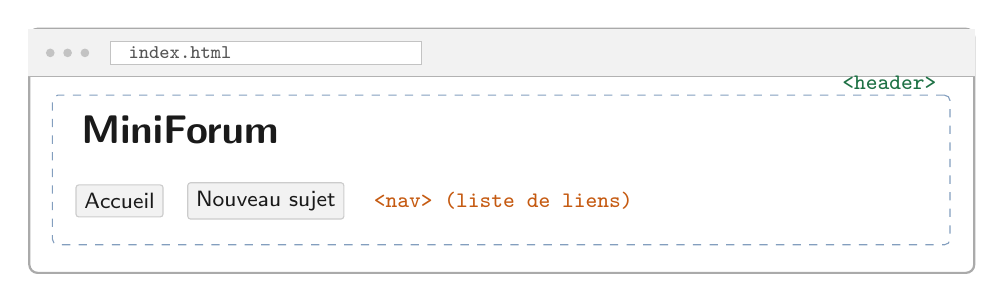
\begin{tikzpicture}[font=\small,
  browser/.style={draw=cfptDarkGrey!50, thick, rounded corners=3pt},
  zone/.style={draw=accentBlue!55, thin, dashed, rounded corners=2pt},
  tag/.style={font=\ttfamily\footnotesize\color{accentBlue}, anchor=west},
  gtag/.style={font=\ttfamily\footnotesize\color{successGreen}, anchor=west},
  content/.style={anchor=west, text=cfptBlack}]
  \node[browser, minimum width=12cm, minimum height=3.1cm, anchor=north] (win) at (0,0) {};
  \browserbar{win}
  % header zone
  \node[zone, minimum width=11.4cm, minimum height=1.9cm, anchor=north west] (hd) at ([xshift=0.3cm, yshift=-0.85cm]win.north west) {};
  \node[content, font=\bfseries\Large] at ([xshift=0.25cm, yshift=-0.45cm]hd.north west) {MiniForum};
  \node[gtag] at ([xshift=-1.5cm, yshift=0.15cm]hd.north east) {<header>};
  % nav
  \node[content, anchor=west, draw=cfptDarkGrey!30, fill=cfptGrey, rounded corners=1pt, inner sep=3pt, font=\footnotesize] (n1) at ([xshift=0.3cm, yshift=-1.35cm]hd.north west) {Accueil};
  \node[content, anchor=west, draw=cfptDarkGrey!30, fill=cfptGrey, rounded corners=1pt, inner sep=3pt, font=\footnotesize, right=0.3cm of n1] (n2) {Nouveau sujet};
  \node[tag, color=warningOrange] at ([xshift=0.25cm]n2.east) {<nav> (liste de liens)};
\end{tikzpicture}
\end{center}

\begin{tcolorbox}[definition, title={À produire}]
Un \texttt{<header>} contenant : un titre \texttt{<h1>} « MiniForum », puis un \texttt{<nav>} avec une liste \texttt{<ul>} de deux liens --- « Accueil » (vers \texttt{index.html}) et « Nouveau sujet » (vers \texttt{\#nouveau-sujet}).
\end{tcolorbox}

\begin{tcolorbox}[astuce, title={Le lien avec le \#}]
Le lien \texttt{href="\#nouveau-sujet"} est un \textbf{lien interne} : il pointera vers l'élément de la page dont l'\texttt{id} est \texttt{nouveau-sujet} (notre formulaire, plus bas). Clique dessus une fois le formulaire créé : la page défilera jusqu'à lui.
\end{tcolorbox}

% ============================================================
\section{La liste des sujets}
% ============================================================

C'est le cœur de la page d'accueil. Chaque sujet du forum est un \texttt{<article>} : rappelle-toi, un article a du sens tout seul, sorti de son contexte.

Dans le \texttt{<main>}, tu vas ajouter une première \texttt{<section>} contenant deux ou trois sujets codés en dur. Voici le \textbf{rendu attendu} :

\vspace{4pt}
\begin{center}
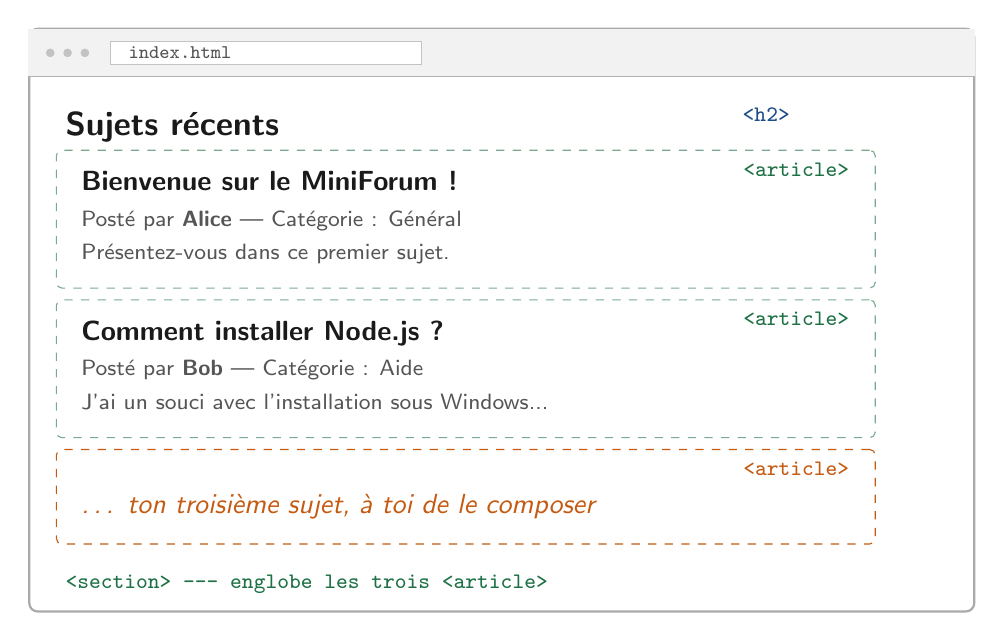
\begin{tikzpicture}[font=\small,
  browser/.style={draw=cfptDarkGrey!50, thick, rounded corners=3pt},
  zone/.style={draw=successGreen!60, thin, dashed, rounded corners=2pt},
  tag/.style={font=\ttfamily\footnotesize, anchor=west},
  content/.style={anchor=north west, text=cfptBlack}]
  \node[browser, minimum width=12cm, minimum height=7.4cm, anchor=north] (win) at (0,0) {};
  \browserbar{win}
  \begin{scope}[shift={([xshift=0.35cm, yshift=-0.95cm]win.north west)}]
    \node[content, font=\bfseries\large] (h2) at (0,0) {Sujets récents};
    \node[tag, color=accentBlue] at (8.6,-0.15) {<h2>};
    % article 1
    \node[zone, minimum width=10.4cm, minimum height=1.75cm, anchor=north west] (a1) at (0,-0.6) {};
    \node[content, font=\bfseries] at (0.2,-0.75) {Bienvenue sur le MiniForum !};
    \node[content, font=\footnotesize, text=cfptDarkGrey] at (0.2,-1.25) {Posté par \textbf{Alice} — Catégorie : Général};
    \node[content, font=\footnotesize, text=cfptDarkGrey] at (0.2,-1.68) {Présentez-vous dans ce premier sujet.};
    \node[tag, color=successGreen, anchor=east] at (10.2,-0.85) {<article>};
    % article 2
    \node[zone, minimum width=10.4cm, minimum height=1.75cm, anchor=north west] (a2) at (0,-2.5) {};
    \node[content, font=\bfseries] at (0.2,-2.65) {Comment installer Node.js ?};
    \node[content, font=\footnotesize, text=cfptDarkGrey] at (0.2,-3.15) {Posté par \textbf{Bob} — Catégorie : Aide};
    \node[content, font=\footnotesize, text=cfptDarkGrey] at (0.2,-3.58) {J'ai un souci avec l'installation sous Windows...};
    \node[tag, color=successGreen, anchor=east] at (10.2,-2.75) {<article>};
    % article 3 à compléter
    \node[zone, draw=warningOrange, minimum width=10.4cm, minimum height=1.2cm, anchor=north west] (a3) at (0,-4.4) {};
    \node[content, font=\itshape, text=warningOrange] at (0.2,-4.85) {\dots\ ton troisième sujet, à toi de le composer};
    \node[tag, color=warningOrange, anchor=east] at (10.2,-4.65) {<article>};
  \end{scope}
  \node[font=\ttfamily\footnotesize\color{successGreen}, anchor=south west] at ([xshift=0.35cm, yshift=0.12cm]win.south west) {<section> --- englobe les trois <article>};
\end{tikzpicture}
\end{center}

\begin{tcolorbox}[definition, title={À produire}]
Une \texttt{<section>} avec un titre \texttt{<h2>} « Sujets récents », puis \textbf{trois} \texttt{<article>}. Dans chaque article : un titre \texttt{<h3>}, une ligne d'information (auteur en \texttt{<strong>} et catégorie), et un paragraphe \texttt{<p>} de contenu.
\end{tcolorbox}

\begin{tcolorbox}[attention, title={« Codé en dur » --- pourquoi ?}]
Ces sujets sont écrits directement dans le HTML : ils ne viennent d'aucune base de données. À ce stade, si tu rafraîchis ou relances la page, ce sont \textbf{toujours les mêmes}. C'est la limite volontaire de la phase 1 : elle rend évident, plus tard, le besoin d'une vraie base de données.
\end{tcolorbox}

% ============================================================
\section{Le formulaire d'ajout de message}
% ============================================================

Sous la liste des sujets, toujours dans le \texttt{<main>}, on ajoute une seconde \texttt{<section>} contenant le formulaire de création de sujet. Cette section portera l'attribut \texttt{id="nouveau-sujet"} (la cible du lien de navigation). Voici le \textbf{rendu attendu} :

\vspace{4pt}
\begin{center}
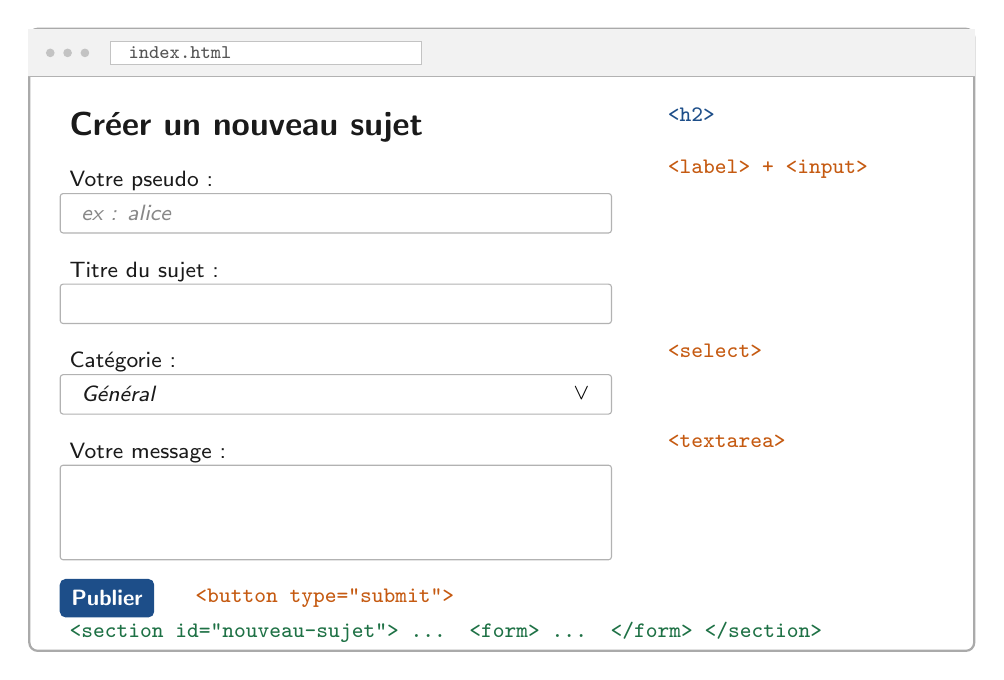
\begin{tikzpicture}[font=\small,
  browser/.style={draw=cfptDarkGrey!50, thick, rounded corners=3pt},
  field/.style={draw=cfptDarkGrey!45, fill=white, rounded corners=1pt, minimum height=0.5cm, anchor=north west},
  lab/.style={anchor=north west, text=cfptBlack, font=\footnotesize},
  tag/.style={font=\ttfamily\footnotesize\color{accentBlue}, anchor=west},
  ph/.style={anchor=west, font=\footnotesize\itshape, text=cfptDarkGrey!70}]
  \node[browser, minimum width=12cm, minimum height=7.9cm, anchor=north] (win) at (0,0) {};
  \browserbar{win}
  \begin{scope}[shift={([xshift=0.4cm, yshift=-0.95cm]win.north west)}]
    \node[lab, font=\bfseries\large] (h2) at (0,0) {Créer un nouveau sujet};
    \node[tag] at (7.6,-0.15) {<h2>};

    % pseudo
    \node[lab] (l1) at (0,-0.75) {Votre pseudo :};
    \node[tag, color=warningOrange] at (7.6,-0.85) {<label> + <input>};
    \node[field, minimum width=7cm] (f1) at (0,-1.15) {};
    \node[ph] at (0.15,-1.4) {ex : alice};

    % titre
    \node[lab] (l2) at (0,-1.9) {Titre du sujet :};
    \node[field, minimum width=7cm] (f2) at (0,-2.3) {};

    % catégorie (select)
    \node[lab] (l3) at (0,-3.05) {Catégorie :};
    \node[tag, color=warningOrange] at (7.6,-3.15) {<select>};
    \node[field, minimum width=7cm] (f3) at (0,-3.45) {};
    \node[ph, text=cfptBlack] at (0.15,-3.7) {Général};
    \node[anchor=east, font=\footnotesize] at (6.85,-3.7) {$\vee$};

    % message (textarea)
    \node[lab] (l4) at (0,-4.2) {Votre message :};
    \node[tag, color=warningOrange] at (7.6,-4.3) {<textarea>};
    \node[field, minimum width=7cm, minimum height=1.2cm] (f4) at (0,-4.6) {};

    % bouton
    \node[draw=accentBlue, fill=accentBlue, text=white, rounded corners=2pt, inner sep=4pt, font=\footnotesize\bfseries, anchor=north west] (btn) at (0,-6.05) {Publier};
    \node[tag, color=warningOrange] at (1.6,-6.3) {<button type="submit">};
  \end{scope}
  \node[font=\ttfamily\footnotesize\color{successGreen}, anchor=south west] at ([xshift=0.4cm, yshift=0cm]win.south west) {<section id="nouveau-sujet"> ... <form> ... </form> </section>};
\end{tikzpicture}
\end{center}

\begin{tcolorbox}[definition, title={À produire}]
Une \texttt{<section id="nouveau-sujet">} avec un \texttt{<h2>} et un \texttt{<form>} contenant, chacun avec son \texttt{<label>} : un champ \textbf{pseudo} (\texttt{text}, avec \texttt{placeholder} et \texttt{required}), un champ \textbf{titre} (\texttt{text}, \texttt{required}), une liste déroulante \textbf{catégorie} (\texttt{<select>} avec les options Général / Aide / Projets), une zone \textbf{message} (\texttt{<textarea>}, \texttt{maxlength} et \texttt{required}), et un \texttt{<button type="submit">} « Publier ».
\end{tcolorbox}

\begin{tcolorbox}[attention, title={Le formulaire ne « part » nulle part}]
Clique sur \textbf{Publier} : rien ne se passe (ou la page se recharge). C'est normal --- il manque le serveur qui recevra les données, prévu pour la \textbf{phase 3}. Vérifie en revanche que la \textbf{validation HTML5} fonctionne : laisse un champ \texttt{required} vide et clique sur Publier, le navigateur doit bloquer l'envoi.
\end{tcolorbox}

% ============================================================
\section{Le pied de page}
% ============================================================

\vspace{2pt}
\begin{center}
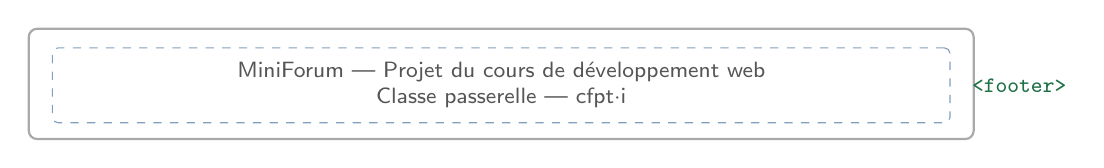
\begin{tikzpicture}[font=\small]
  \node[draw=cfptDarkGrey!50, thick, rounded corners=3pt, minimum width=12cm, minimum height=1.4cm, anchor=north] (win) at (0,0) {};
  \node[draw=accentBlue!55, thin, dashed, rounded corners=2pt, minimum width=11.4cm, minimum height=0.95cm, anchor=north] (fz) at ([yshift=-0.25cm]win.north) {};
  \node[anchor=center, font=\footnotesize, text=cfptDarkGrey, align=center] at (fz.center) {MiniForum --- Projet du cours de développement web\\ Classe passerelle --- cfpt$\cdot$i};
  \node[font=\ttfamily\footnotesize\color{successGreen}, anchor=east] at ([xshift=-0.15cm]fz.east) {};
  \node[font=\ttfamily\footnotesize\color{successGreen}, anchor=west] at ([xshift=0.15cm]fz.east) {<footer>};
\end{tikzpicture}
\end{center}

\begin{tcolorbox}[definition, title={À produire}]
Un \texttt{<footer>} avec deux paragraphes \texttt{<p>} : le nom du projet, et la mention de la classe.
\end{tcolorbox}

% ============================================================
\section{Valider et sauvegarder}
% ============================================================

\subsection{Valider le HTML}

\begin{enumerate}
  \item Aller sur \texttt{validator.w3.org}, onglet \textit{Validate by Direct Input}.
  \item Copier-coller tout le contenu de \texttt{index.html}, puis cliquer sur \textit{Check}.
  \item Corriger les éventuelles erreurs signalées (balise mal fermée, \texttt{alt} manquant\dots) jusqu'à obtenir un résultat \textbf{sans erreur}.
\end{enumerate}

\begin{tcolorbox}[astuce, title={Erreurs fréquentes}]
Les plus courantes : une balise ouverte mais jamais fermée, un \texttt{id} utilisé deux fois sur la même page, ou un attribut \texttt{for} de \texttt{<label>} qui ne correspond à aucun \texttt{id}. Le validateur indique la ligne : lis le message, il est souvent explicite.
\end{tcolorbox}

\subsection{Sauvegarder sur GitHub}

Dans la continuité du TP de la semaine 1, on enregistre le travail et on l'envoie sur GitHub.

\begin{lstlisting}[language=bash]
git add .
git commit -m "Squelette HTML du MiniForum : sujets et formulaire"
git push
\end{lstlisting}

\begin{tcolorbox}[astuce, title={Le bon réflexe}]
Prends l'habitude de committer à chaque étape terminée, avec un message clair, et de pousser en fin de séance. Rafraîchis la page de ton dépôt sur \texttt{github.com} : ton \texttt{index.html} mis à jour doit y apparaître.
\end{tcolorbox}

% ============================================================
\section{Pour aller plus loin (optionnel)}
% ============================================================

Si tu as terminé en avance, voici de quoi enrichir ta page :

\begin{itemize}
  \item Ajouter une image de logo dans le \texttt{<header>} avec la balise \texttt{<img>} (sans oublier l'attribut \texttt{alt}).
  \item Transformer la liste des catégories en un vrai \texttt{<nav>} secondaire.
  \item Ajouter un champ \texttt{type="email"} au formulaire et tester la validation automatique du navigateur.
  \item Ajouter un attribut \texttt{maxlength} au champ « titre » pour limiter sa longueur.
\end{itemize}

% ============================================================
\section{Points de contrôle}
% ============================================================

\begin{tcolorbox}[definition, title={Auto-évaluation}]
\begin{itemize}
  \item[$\square$] La page a une structure sémantique : \texttt{<header>}, \texttt{<main>}, \texttt{<footer>}
  \item[$\square$] L'en-tête contient un \texttt{<h1>} et une navigation \texttt{<nav>}
  \item[$\square$] Le \texttt{<main>} affiche au moins \textbf{trois} sujets, chacun dans un \texttt{<article>}
  \item[$\square$] Le formulaire contient pseudo, titre, catégorie et message, avec leurs \texttt{<label>}
  \item[$\square$] Chaque \texttt{<label>} est relié à son champ (\texttt{for} / \texttt{id})
  \item[$\square$] Les champs obligatoires ont l'attribut \texttt{required} (validation testée)
  \item[$\square$] La page passe \texttt{validator.w3.org} \textbf{sans erreur}
  \item[$\square$] Le travail est poussé sur GitHub avec un message de commit clair
\end{itemize}
\end{tcolorbox}

\vspace{6pt}
\begin{tcolorbox}[attention, title={À rendre avant la semaine 3}]
Le dépôt GitHub \texttt{miniforum} mis à jour, avec le squelette HTML validé. La semaine 3 introduira le \textbf{CSS} pour donner enfin du style à cette structure.
\end{tcolorbox}

\end{document}
